%%%%%%%%%%%%%%%%%%%%%%%%%%%%%%%%%%%%%%%%%
% Focus Beamer Presentation
% LaTeX Template
% Version 1.0 (8/8/18)
%
% This template has been downloaded from:
% http://www.LaTeXTemplates.com
%
% Original author:
% Pasquale Africa (https://github.com/elauksap/focus-beamertheme) with modifications by 
% Vel (vel@LaTeXTemplates.com)
%
% Template license:
% GNU GPL v3.0 License
%
% Important note:
% The bibliography/references need to be compiled with bibtex.
%
%%%%%%%%%%%%%%%%%%%%%%%%%%%%%%%%%%%%%%%%%

%----------------------------------------------------------------------------------------
%	PACKAGES AND OTHER DOCUMENT CONFIGURATIONS
%----------------------------------------------------------------------------------------

\documentclass{beamer}

\usetheme{focus} % Use the Focus theme supplied with the template
% Add option [numbering=none] to disable the footer progress bar
% Add option [numbering=fullbar] to show the footer progress bar as always full with a slide count

% Uncomment to enable the ice-blue theme
%\definecolor{main}{RGB}{92, 138, 168}
%\definecolor{background}{RGB}{240, 247, 255}
\definecolor{main}{RGB}{255, 71, 133}
\definecolor{background}{RGB}{0, 13, 26}

%Define the listing package
\usepackage{listings} %code highlighter
%\usepackage{color} %use color
\definecolor{mygreen}{rgb}{0,0.6,0}
\definecolor{mygray}{rgb}{0.5,0.5,0.5}
\definecolor{mymauve}{rgb}{0.58,0,0.82}
 
%Customize a bit the look
\lstset{ %
backgroundcolor=\color{white}, % choose the background color; you must add \usepackage{color} or \usepackage{xcolor}
basicstyle=\footnotesize, % the size of the fonts that are used for the code
breakatwhitespace=false, % sets if automatic breaks should only happen at whitespace
breaklines=true, % sets automatic line breaking
captionpos=b, % sets the caption-position to bottom
commentstyle=\color{mygreen}, % comment style
deletekeywords={...}, % if you want to delete keywords from the given language
escapeinside={\%*}{*)}, % if you want to add LaTeX within your code
extendedchars=true, % lets you use non-ASCII characters; for 8-bits encodings only, does not work with UTF-8
frame=single, % adds a frame around the code
keepspaces=true, % keeps spaces in text, useful for keeping indentation of code (possibly needs columns=flexible)
keywordstyle=\color{blue}, % keyword style
% language=Octave, % the language of the code
morekeywords={*,...}, % if you want to add more keywords to the set
numbers=left, % where to put the line-numbers; possible values are (none, left, right)
numbersep=5pt, % how far the line-numbers are from the code
numberstyle=\tiny\color{mygray}, % the style that is used for the line-numbers
rulecolor=\color{black}, % if not set, the frame-color may be changed on line-breaks within not-black text (e.g. comments (green here))
showspaces=false, % show spaces everywhere adding particular underscores; it overrides 'showstringspaces'
showstringspaces=false, % underline spaces within strings only
showtabs=false, % show tabs within strings adding particular underscores
stepnumber=1, % the step between two line-numbers. If it's 1, each line will be numbered
stringstyle=\color{mymauve}, % string literal style
tabsize=2, % sets default tabsize to 2 spaces
title=\lstname % show the filename of files included with \lstinputlisting; also try caption instead of title
}
%END of listing package%
 
\definecolor{darkgray}{rgb}{.4,.4,.4}
\definecolor{purple}{rgb}{0.65, 0.12, 0.82}
 
%define Javascript language
\lstdefinelanguage{JavaScript}{
keywords={typeof, new, true, false, catch, function, return, null, catch, switch, var, if, in, while, do, else, case, break},
keywordstyle=\color{blue}\bfseries,
ndkeywords={class, export, boolean, throw, implements, import, this},
ndkeywordstyle=\color{darkgray}\bfseries,
identifierstyle=\color{black},
sensitive=false,
comment=[l]{//},
morecomment=[s]{/*}{*/},
commentstyle=\color{purple}\ttfamily,
stringstyle=\color{red}\ttfamily,
morestring=[b]',
morestring=[b]"
}
 
\lstset{
language=JavaScript,
extendedchars=true,
basicstyle=\footnotesize\ttfamily,
showstringspaces=false,
showspaces=false,
numbers=left,
numberstyle=\footnotesize,
numbersep=9pt,
tabsize=2,
breaklines=true,
showtabs=false,
captionpos=b
} %Eigene lstlisting Erweiterung

%------------------------------------------------

\usepackage{booktabs} % Required for better table rules

%----------------------------------------------------------------------------------------
%	 TITLE SLIDE
%----------------------------------------------------------------------------------------

\title{Storybook}

\subtitle{UI component explorer for frontend developers}

\author{Gimleux}

\titlegraphic{
\includegraphics[scale=.3]{Images/storybook_logo.png}} % Optional title page image, comment this line to remove it

\institute{Software Engineering}

\date{June 01, 2021}

%------------------------------------------------

\begin{document}

%------------------------------------------------

\begin{frame}
	\maketitle % Automatically created using the information in the commands above
\end{frame}

%----------------------------------------------------------------------------------------
%	 Was ist Storybook
%----------------------------------------------------------------------------------------

\section{Was ist Storybook?} % Section title slide, unnumbered

\begin{frame}{Was ist Storybook?}
	\begin{columns}
		\column{0.7\textwidth}
		\begin{itemize}
			\item Hilfsmittel bei frontendseitiger Web-Entwicklung
			\item Isolierte Entwicklung von Web-Komponenten
			\begin{itemize}
				\item \emph{component-driven-development}
			\end{itemize}
		\end{itemize}
		
		\column{0.3\textwidth}
		
\includegraphics[width=\linewidth]{Images/storybook_logo.png}
	\end{columns}
\end{frame}

\begin{frame}{Was ist eine Story?}
	\begin{itemize}
		\item Beschreibt markanten/interessanten Zustand einer Web-Komponente
			\begin{itemize}
				\item In bestimmten Zuständen
				\item Bei bestimmten Ereignissen
				\item Mit bestimmtem Design
				\item ...
			\end{itemize}
		\item Für eine Web-Komponente sind beliebig viele Stories implementierbar
	\end{itemize}
\end{frame}

%----------------------------------------------------------------------------------------
%	 Vorteile
%----------------------------------------------------------------------------------------

\section{Was sind die Vorteile?} % Section title slide, unnumbered

\begin{frame}{Was sind die Vorteile?}
	\begin{itemize}
		\item Erlaubt an einer einzelnen Komponente zu arbeiten, ohne gesamte Webseite berühren und berücksichtigen zu müssen
		\begin{itemize}
			\item Einfachere \& schnellere Entwicklung der Komponente
			\item Geringere Fehleranfälligkeit
		\end{itemize}
		\item Nutzung von Testdaten innerhalb der Komponente, ohne Einbindung des restlichen Systems
		\item Automatische Dokumentation
	\end{itemize}
\end{frame}

\begin{frame}{Was sind die Vorteile?}
	\begin{itemize}
		\item Isolierte Darstellung von Web-Komponenten
		\item Veränderbarkeit der Komponente über Web-Oberfläche
		\begin{itemize}
			\item Isolierte Präsentation für Product Owner
			\item Simple Live-Anpassungen mit oder durch Product Owner
			\begin{itemize}
				\item => Vereinfachte Zusammenarbeit (intern \& extern)
			\end{itemize}
		\end{itemize}
	\end{itemize}
\end{frame}

\begin{frame}{Was sind die Vorteile?}
	\begin{itemize}
		\item Einzelne Komponenten lassen sich per iFrame einbetten
		\includegraphics[scale=.5]{Images/interactive_demo.png}
	\end{itemize}
\end{frame}

%----------------------------------------------------------------------------------------
%	 Logik hinter Storybook
%----------------------------------------------------------------------------------------
\section{Logik in Storybook} % Section title slide, unnumbered

\begin{frame}{".storybook"-Ordner}
	\begin{columns}	
		\column{0.5\textwidth}
		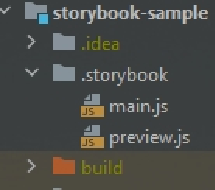
\includegraphics{Images/file/storybook-project-folder.pdf}
		
		\column{0.5\textwidth}
		".storybook"-Ordner
		\begin{itemize}
			\item Wird bei Installation angelegt
			\item Enthält Grund- und ggf. Add-On-Einstellungen
		\end{itemize}
	\end{columns}
\end{frame}

\begin{frame}{Dateistruktur einer Komponente}
	\begin{columns}	
		\column{0.5\textwidth}
		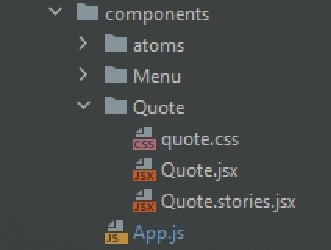
\includegraphics{Images/file/storybook-component-folder.pdf}
		
		\column{0.5\textwidth}
		\begin{itemize}
			\item Storybook-Dateien enthalten den String "\alert{.stories.}"
			\item Best Practice: <Komponentenname> \alert{.stories.}{}<Typ>
		\end{itemize}
	\end{columns}
\end{frame}

\begin{frame}[fragile]{Aufbau einer Storybook-Datei}
	\begin{itemize}
		\item Import von React sowie der eigentlichen Komponente
	\end{itemize}
	\begin{lstlisting}[language=JavaScript]
		import React from 'react';
		import {Button} from './Button';
	\end{lstlisting}		
\end{frame}

\begin{frame}[fragile]{Aufbau einer Storybook-Datei}
	\begin{itemize}
		\item Storybook-Objekt erstellen
	\end{itemize}
	\begin{lstlisting}[language=JavaScript]
		export default {
			title: 'Atoms/Button',
			component: Button,
			argTypes: {
				color: {control: "color"},
				backgroundColor: {control: 'color'},
			},
		};
	\end{lstlisting}
\end{frame}

\begin{frame}[fragile]{Aufbau einer Storybook-Datei}
	\begin{itemize}
		\item Erstellung eines Templates für die Komponente
		\begin{itemize}
			\item Template kann beliebig über die eigentliche Komponente hinaus erweitert werden
		\end{itemize}
	\end{itemize}
	\begin{lstlisting}[language=JavaScript]
		const Template = (args) => <Button {...args} />;
	\end{lstlisting}
	\begin{lstlisting}[language=JavaScript]
		const CenteredTemplate = (args) => (
		<div className="flex-centered">
		<Button {...args} />
		</div>
		);
	\end{lstlisting}
\end{frame}

\begin{frame}[fragile]{Aufbau einer Storybook-Datei}
	\begin{itemize}
		\item Erstellung von Stories
	\end{itemize}
	\begin{lstlisting}[language=JavaScript]
		export const Default = Template.bind({});
	\end{lstlisting}
	\begin{lstlisting}[language=JavaScript]
		export const NotPrimary = Template.bind({});
		NotPrimary.args = {
			isPrimary: false
		};
	\end{lstlisting}
	\begin{lstlisting}[language=JavaScript]
		export const Large = Template.bind({});
		Large.args = {
			size: 'large'
		};
	\end{lstlisting}
\end{frame}

\begin{frame}[fragile]{Parameter-Typisierung}
	\begin{itemize}
		\item Angabe der erwarteten Argumente und eventueller default-Werte
	\end{itemize}
	\begin{lstlisting}[language=JavaScript]
		Button.propTypes = {
			/**
			* Is this the principal call to action on the page?
			*/
			isPrimary: PropTypes.bool,
			/**
			* How large should the button be?
			*/
			size: PropTypes.oneOf(['small', 'medium', 'large']),
		};
	
		Button.defaultProps = {
			isPrimary: false,
			size: 'medium',
		};
	\end{lstlisting}
\end{frame}

%----------------------------------------------------------------------------------------
%	 Web-Oberfläche
%----------------------------------------------------------------------------------------
\section{Aufbau der Web-Oberfläche} % Section title slide, unnumbered

\begin{frame}{Aufbau der Web-Oberfläche}
	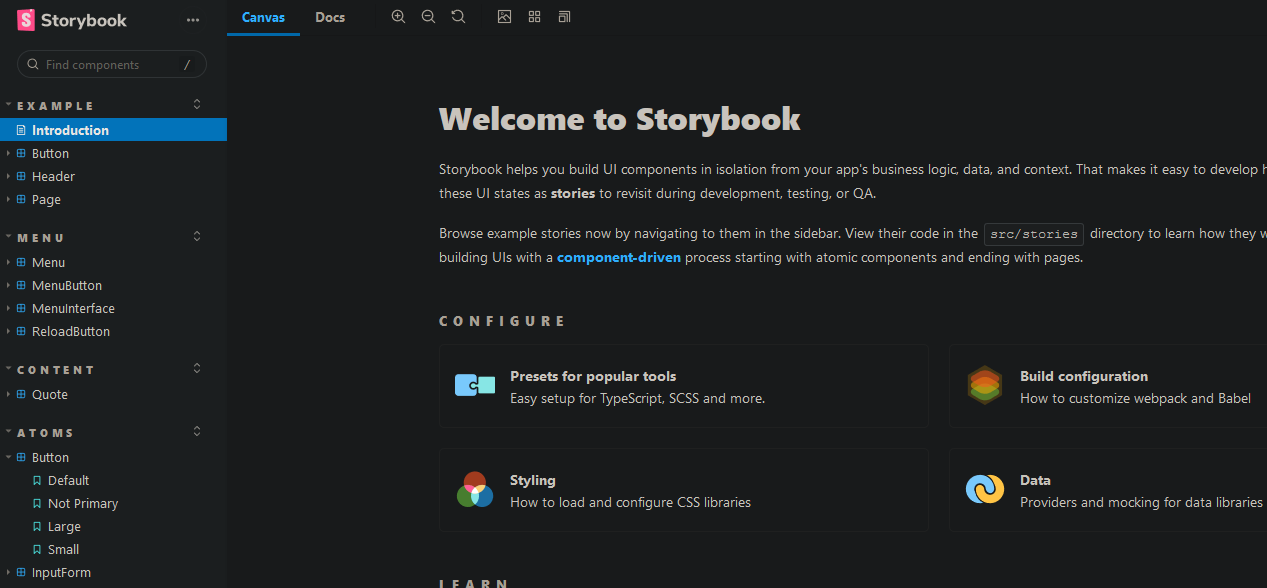
\includegraphics[width=\textwidth]{Images/web-ui/whole-ui.png}
\end{frame}

\begin{frame}{Seitenleiste}
	\begin{columns}
		\column{0.5\textwidth}
		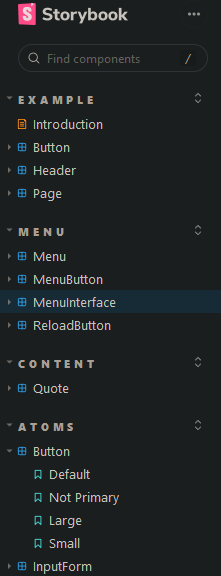
\includegraphics[height=.8\textheight]{Images/web-ui/sidebar.png}
		
		\column{0.5\textwidth}
		Unterteilung in
		\begin{itemize}
			\item Bereiche (z.B. Atoms)
			\item Komponenten (z.B. Button)
			\item Stories (z.B. Large)
		\end{itemize}
	\end{columns}
\end{frame}

\begin{frame}{Canvas}
	\begin{columns}
		\column{0.5\textwidth}
		\begin{itemize}
			\item Ansicht der Komponente
			\item Kontrollbereich, über welchen die Komponente direkt verändert werden kann
		\end{itemize}
		
		\column{0.5\textwidth}
		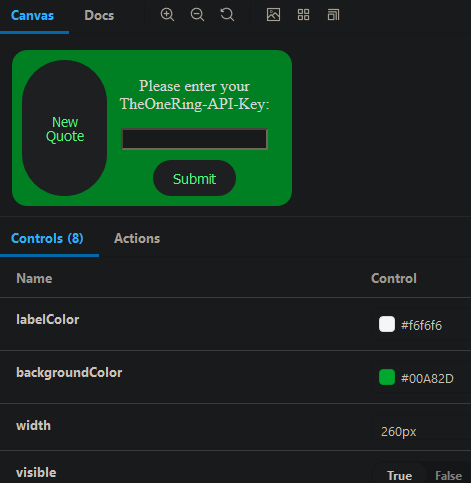
\includegraphics[width=\linewidth]{Images/web-ui/canvas.png}
	\end{columns}
\end{frame}

\begin{frame}{Docs}
	\begin{columns}
		\column{0.5\textwidth}
		\begin{itemize}
			\item Übersicht der Komponente, ihrer Stories und Parameter
			\item Einsicht des zur Implementierung benötigten Codes
			\item Details zu Parametern der Komponente
		\end{itemize}
		
		\column{0.5\textwidth}
		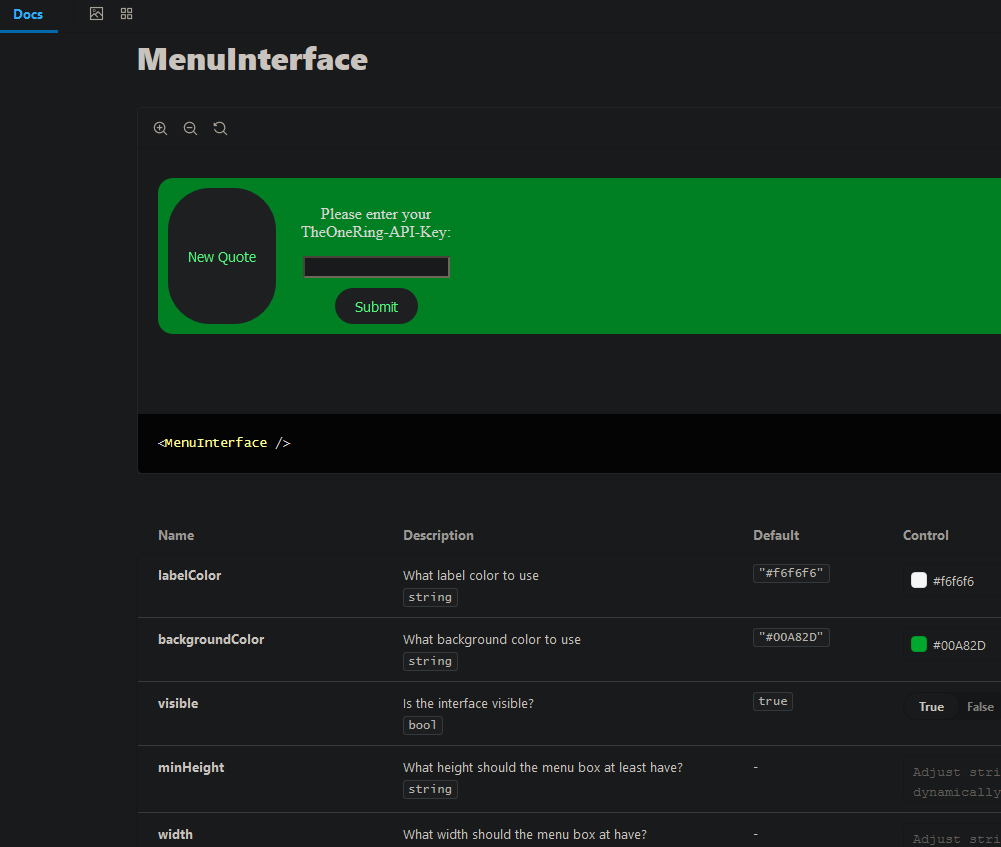
\includegraphics[width=\linewidth]{Images/web-ui/docs.png}
	\end{columns}
\end{frame}

%----------------------------------------------------------------------------------------
%	 Aufsetzen
%----------------------------------------------------------------------------------------
\section{Projekt-Initialisierung} % Section title slide, unnumbered

\begin{frame}{Projekt initialisieren}
	\begin{itemize}
		\item npx create-react-app [--use-npm]
		\item npx sb init
	\end{itemize}
\end{frame}

\begin{frame}{Storybook ausführen}
	\begin{itemize}
		\item cd create-react-app
		\item npm run storybook
	\end{itemize}
\end{frame}

%----------------------------------------------------------------------------------------
%	 Live-Coding
%----------------------------------------------------------------------------------------
\section{Live-Coding} % Section title slide, unnumbered

%------------------------------------------------

%----------------------------------------------------------------------------------------
%	 CLOSING/SUPPLEMENTARY SLIDES
%----------------------------------------------------------------------------------------

\appendix

%------------------------------------------------

%\begin{frame}{Backup Slide}
%	This is a backup slide, useful to include additional materials to answer questions from the audience.
%	\vfill
%	The package \texttt{appendixnumberbeamer} is used to refrain from numbering appendix slides.
%\end{frame}

%----------------------------------------------------------------------------------------

\end{document}
